\documentclass[useAMS,usenatbib]{mn2e}                                  
%
%\def\del#1{{\bf  [deleted text] }} \def\new#1{{\bf #1}} \def\remark#1{{\bf  [remark: #1]}}
%\def\del#1{} \def\new#1{#1} \def\remark#1{}

\def\del#1{{}}
%\def\del#1{{\bf (DELETED TEXT)}}
\def\C#1{{\bf #1}}
%\def\C#1{#1}

%\newcommand{\rmn}{\mathrm}
\newcommand{\CR}{\mathrm{CR}}
\newcommand{\expval}[1]{\left\langle #1 \right\rangle}
\newcommand{\RA}[3]{#1$^{\mathrm{h}}$#2$^{\mathrm{m}}$#3$^{\mathrm{s}}$}
\newcommand{\Dec}[3]{#1$^{\circ}$#2\arcmin#3\arcsec}
\newcommand{\dps}{\displaystyle}
\newcommand{\eps}{\varepsilon}
\newcommand{\dd}{\mathrm{d}}
\newcommand{\vel}{\upsilon}
%
\usepackage{graphicx}
\usepackage{natbib}
%
\usepackage{txfonts}

%\voffset-0.5in

%MNRAS
\title[A Phenomenological Model for the Intra-Cluster Medium]{A Phenomenological Model for the Intra-Cluster Medium that matches X-ray and Sunyaev-Zel'dovich observations}
\author[F. Zandanel, C. Pfrommer and F. Prada]{
Fabio Zandanel$^{1,2 *}$, Christoph Pfrommer$^{3 \dagger}$ and Francisco Prada$^{4,5,1 \S}$\\
$^{1}$Instituto de Astrof\'{\i}sica de Andaluc\'{\i}a (CSIC), Glorieta de la Astronom\'{\i}a, E-18080 Granada, Spain\\
$^{2}$now at GRAPPA Institute, University of Amsterdam, Science Park 904, 1098XH Amsterdam, Netherlands\\
$^{3}$Heidelberg Institute for Theoretical Studies, Schloss-Wolfsbrunnenweg 35, D-69118 Heidelberg, Germany\\
$^{4}$Campus of International Excellence UAM+CSIC, Cantoblanco, E-28049 Madrid, Spain\\
$^{5}$Instituto de F\'{\i}sica Te\'orica, (UAM/CSIC), Universidad Aut\'onoma de Madrid, Cantoblanco, E-28049 Madrid, Spain}
\begin{document}

\date{Accepted XXX. Received XXX; in original from XXX}

\pagerange{\pageref{firstpage}--\pageref{lastpage}} \pubyear{2012}

\maketitle

\label{firstpage}

%%%%%%%%%%%%%%%%%%%%%%%%%%%%%%%%%%%%%%%
\begin{abstract}
  ...
  We build a mock galaxy cluster catalog from the large MultiDark $N$-body $\Lambda$CDM 
  simulation by adopting a phenomenological gas density model for each cluster based on X-ray
  measurements that matches Sunyaev-Zel'dovich and X-ray scaling relations and
  luminosity function. 
  ...
  We make our cosmologically complete multi-frequency mock catalogs for 
  the (non-)thermal cluster emission at different redshifts publicly and freely available on-line
  through the MultiDark database.
\end{abstract}

\begin{keywords}
  Galaxies: clusters: intracluster medium - X-rays: galaxies: clusters - astronomical data bases: catalogues
\end{keywords}



%%%%%%%%%%%%%%%%%%%%%%%%%%%%%%%%%%%%%%%%%%%%%%%%%%%%%%%%%%%%%%%%%%%
%%%%%%%%%%%%%%%%%%%%%%%%%%%%%%%%%%%%%%%%%%%%%%%%%%%%%%%%%%%%%%%%%%%
\section{Introduction}
\label{sec:1}

\begingroup
\let\thefootnote\relax\footnotetext{* f.zandanel@uva.nl}
\let\thefootnote\relax\footnotetext{$\dagger$ christoph.pfrommer@h-its.org}
\let\thefootnote\relax\footnotetext{$\S$ fprada@iaa.es}
\endgroup

{\bf Introduction...}

%
%dark matter (DM)  
%

{\bf Our original motivation to build such a mock catalog is to predict the 
non-thermal emission at radio and gamma-ray frequencies of a cosmological 
complete sample of galaxy clusters. This is presented in a companion 
paper (REF, hereafter Paper~2).
The two basic ingredients of the two works are an $N$-body, \emph{DM-only}
cosmological simulation that we use in constructing our complete cluster sample,
and the (non-)thermal emission model. Here, we use the MultiDark simulation that
will be described in Section~\ref{sec:2}, along with our final cluster sample. As described 
in Paper~2, for any given cluster, the necessary ingredients for the non-thermal emission 
model are mass, temperature, and gas density distribution. We assign to
each cluster in that simulation a gas density profile that is phenomenologically
constructed from state-of-art X-ray observations, as will be shown in
Section~\ref{sec:3}. In Section~4 and 5, we will show that this approach can successfully
reproduce the known X-ray cluster characteristics, such as the X-ray luminosity
function (XLF), the luminosity-mass relation, $L_{\rmn{X}}- M$, and the
$Y_{\rmn{X}}-M$ relation, where $Y_{\rmn{X}}=M_\rmn{gas}k_{\rmn{B}}T$ with an
X-ray-derived gas mass $M_{\rmn{gas}}$ and temperature $T$
\citep{2006ApJ...650..128K}. Moreover, we compare our $Y_{\rmn{SZ}}-M$ relation
with SZ-derived measurements. Only if our model matches available cluster data
on the gas properties, we can safely use it in Paper~2.} In this work, the cluster mass $M_{\Delta}$ 
and radius $R_{\Delta}$ are defined with respect to a density that is $\Delta=200$ or 
$\Delta=500$ times the \emph{critical} density of the Universe. We adopt density 
parameters of $\Omega_{\rmn{m}}=0.27$, $\Omega_{\Lambda}=0.73$ and today's 
Hubble constant of $H_0 = 100 \times h_{70}$~km~s$^{-1}$~Mpc$^{-1}$ where $h_{70} = 0.7$.


%%%%%%%%%%%%%%%%%%%%%%%%%%%%%%%%%%%%%%%%%%%%%%%%%%%%%%%%%%%%%%%%%%%
%%%%%%%%%%%%%%%%%%%%%%%%%%%%%%%%%%%%%%%%%%%%%%%%%%%%%%%%%%%%%%%%%%%
\section{MultiDark simulation and final cluster sample}
\label{sec:2}
The MultiDark simulation used in this work is described in detail in \cite{2011arXiv1104.5130P}.  
It is an $N$-body cosmological simulation done with the Adaptive-Refinement-Tree (ART) 
code \citep{1997ApJS..111...73K} of $2048^3$ particles within a ($1000$~Mpc~$h^{-1}$)$^3$ 
cube. The adopted cosmological parameters are $\Omega_{\rmn{m}}=0.27$, $\Omega_{\Lambda}=0.73$,
$\Omega_\rmn{b}=0.0469$, $n_\rmn{s}=0.95$, $h=0.7$ and $\sigma_8=0.82$. This simulation is 
particularly well suited for our purpose because of its large 
number of high-mass objects, i.e., galaxy clusters.
 
We use the MultiDark halo catalog from its on-line database,\footnote{www.multidark.org.} 
constructed with the Bound Density Maxima algorithm \citep{1997astro.ph.12217K}.  
We will mainly use $M_{500}$ and $R_{500}$ for comparison with existing observational works.  
We use the technique described in \cite{2003ApJ...584..702H} to convert $M_{200}$ and
$R_{200}$ provided by the MultiDark halo catalog to $M_{500}$ and $R_{500}$.  In
creating our cluster sample we only select distinct halos, i.e., those halos that
are not sub-halos of any other halo, which by definition are not galaxy clusters.

Additionally, we assume that the main emission mechanism in the ICM is thermal
bremsstrahlung, which is true only above a particle energy of approximately
$2.6$~keV \citep{1988xrec.book.....S}. Below this
energy, there could be other important contributions to the emission,
e.g., from atomic lines. Therefore, we impose a mass cut of
$M_{200}\geq1\times10^{14}$~$h^{-1}$~M$_{\odot}\approx1.4\times10^{14}$~$h_{70}^{-1}$~M$_{\odot}$
which ensures $k_{\rmn{B}}T \gtrsim 2.6$~keV, assuming the $M_{500} - T_{\rmn{ci}}$ relation
of \cite{2010MNRAS.406.1773M}.

{\bf In Paper~2, we present predictions for the LOFAR radio observatory
which is expected to detect diffuse radio emission in clusters up to redshift $z \approx 1$ (e.g.,
\citealp{2012JApA..tmp...34R}).} 
Thus, we make use of different simulation snapshots up to $z=1$. 
{\bf The extrapolation of our model beyond this redshift is rather uncertain as it is based
on observations at low(er) redshift.}
In Table~\ref{tab:z}, we show the total cluster number in our final cluster sample at different redshifts.

\begin{table} 
\begin{center}
\caption{Number of halos in the final cluster sample}
\medskip
\begin{tabular}{cc}
\hline
\phantom{\Big|}
redshift $z$ & number of halos \\
\hline\\[-0.5em]
 0.0~~ &  13763\\
 0.1~~ &  12398\\
 0.2~~ &  10783\\ 
 0.4~~ &   ~~7789\\ 
 0.61  &  ~~5187\\ 
 0.78  &  ~~3372\\ 
 1.0~~ &  ~~1803\\[0.5em]
\hline
\end{tabular}
\label{tab:z}
\end{center}
\footnotesize{Note. We show the number of halos in our MultiDark snapshots at redshift $z$ for $M_{200}\geq1\times10^{14}$~$h^{-1}$~M$_{\odot}\approx1.4\times10^{14}$~$h_{70}^{-1}$~M$_{\odot}$. }
\end{table}


%%%%%%%%%%%%%%%%%%%%%%%%%%%%%%%%%%%%%%%%%%%%%%%%%%%%%%%%%%%%%%%%%%%
%%%%%%%%%%%%%%%%%%%%%%%%%%%%%%%%%%%%%%%%%%%%%%%%%%%%%%%%%%%%%%%%%%%
\section{Gas density modeling}
\label{sec:3}

We decided to use a \emph{phenomenological} approach and to construct the gas
density profiles directly from X-ray observations. A suitable X-ray sample that
provides the needed information is the \emph{Representative XMM-Newton Cluster
  Structure Survey} (REXCESS) sample \citep{2008A&A...487..431C,
  2009A&A...498..361P}. It is a sample of 31 galaxy clusters of different
dynamical states at redshifts $0.06<z<0.18$ with detailed information on the
de-projected electron density profiles \citep{2008A&A...487..431C}. In
Fig.~\ref{fig:gas_profiles}, we show the 31 electron density profiles of the
REXCESS sample color-coded by CCCs and NCCCs.

In order to obtain an electron density profile that we will attach to our
simulated clusters, we use a generalized Navarro-Frank-White (GNFW) profile,
\begin{equation}
n_{\rmn{e}}(x) = \frac{n_{0}}{x^{\beta}\left[1+x^{\alpha}\right]^{\frac{\delta-\beta}{\alpha}}},
\label{eq:gnfw}
\end{equation}
where $x=R/R_{\rmn{c}}$ and $R_{\rmn{c}}$ is the cluster core radius. To reduce
the dimensionality of our fit, we fix representative values of $R_{\rmn{c}} =
0.2\, R_{500}$, $\alpha = 1$ and $\delta = 2.5$. We fit the radial density
profiles of the REXCESS sample in log-log space, separating them in the two
categories of NCCCs and CCCs as shown in Fig.~\ref{fig:gas_profiles}.  We
obtain $n_{\rmn{0,NCCC}} = 1.02\times10^{-2}$~$h_{70}^{1/2}$~cm$^{-3}$,
$n_{\rmn{0,CCC}} = 8.32\times10^{-3}$~$h_{70}^{1/2}$~cm$^{-3}$,
$\beta_{\rmn{NCCC}} = -0.093$, and $\beta_{\rmn{CCC}} = 0.592$. The resulting
fits are shown in blue and red for the NCCC and CCC population, respectively.

The next step is to introduce a mass-scaling in order to apply our GNFW profiles
to all our clusters. We adopt the gas mass fraction-mass scaling,
$f_{\rmn{gas},500}-M_{500}$ of \cite{2009ApJ...693.1142S} (and adopt their equation~(8)). We can
express $f_{\rmn{gas},500}$ in the following way:
\begin{equation}
f_{\rmn{gas},500} = \frac{M_{\rmn{gas},500}}{M_{500}}  = \frac{\int_{0}^{R_{500}} \rho_{\rmn{gas}} \rmn{d}V}{M_{500}}
\label{eq:m500}
\end{equation}
with $\rho_{\rmn{gas}}(R) = \rho_{\rmn{gas}} = n_{\rmn{e}} m_{\rmn{p}} / ( X_{\rmn{H}}X_{\rmn{e}} )$ where
$m_{\rmn{p}}$ is the proton mass, $X_{\rmn{H}} = 0.76$ is the primordial hydrogen
mass fraction and $X_{\rmn{e}} = 1.157$ the ratio of electron-to-hydrogen number
densities in the fully ionized ICM \citep{1988xrec.book.....S}. For each cluster
$i$ of our sample, we then define a \emph{mass-scaled} gas profile as
$\rho_{\rmn{gas},i}=C_{i} \,\rho_{\rmn{gas}}$ with:
\begin{eqnarray}
%C_{i}  =  (0.0616\pm(0.0060g_{1}))  h_{73}^{-1.5}  \left(\frac{M_{500,i}}{10^{13} h_{73}^{-1} \rmn{M_{\odot}}}\right)^{0.135\pm(0.030g_{2})} \nonumber \\
C_{i}  & = &  (0.0656\pm(0.0064g_{1})) \, h_{70}^{-1.5}  \nonumber \\
 & \times & \left(\frac{M_{500,i}}{1.04 \times 10^{13} h_{70}^{-1} \rmn{M_{\odot}}}\right)^{0.135\pm(0.030g_{2})} \frac{M_{500,i}}{\int_{0}^{R_{500,i}} \rho_{\rmn{gas}} \rmn{d}V}
\label{eq:gas_scaling}
\end{eqnarray}
where $g_{1}$ and $g_{2}$ are random Gaussian number which we use in order to
simulate the natural scatter of the gas profiles.\footnote{The values
  $0.0064$ and $0.03$ quoted in equation~(\ref{eq:gas_scaling}) do not represent
  the proper scatter of the $f_{\rmn{gas},500}-M_{500}$ relation but reflect the
  parameter errors and we rescaled the numerical values to a Hubble constant of
  $h_{70}$ used in this work.}

\begin{figure} 
\centering
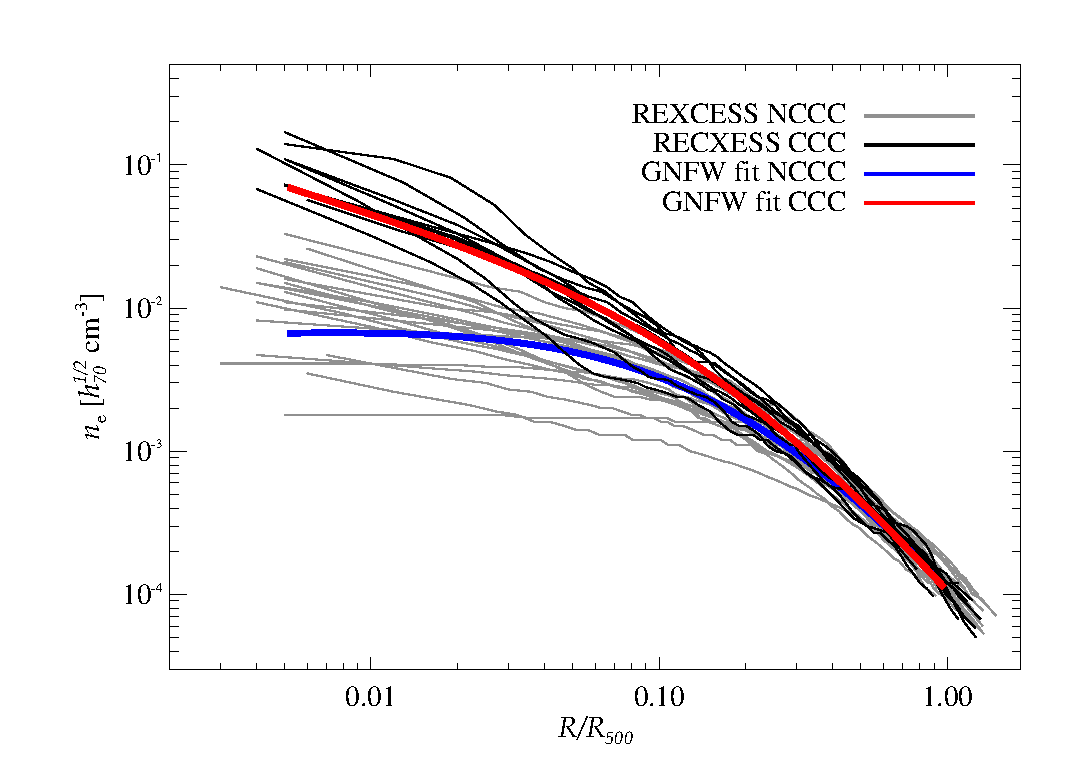
\includegraphics[width=0.48\textwidth]{figures/gas_profiles.eps}
\caption{Electron density profiles of the 31 clusters in the REXCESS sample. Grey and black lines represent NCCCs and CCCs, respectively. The blue and red lines represent our GNFW mean profile for the NCCCs and CCCs, respectively.}
\label{fig:gas_profiles}
\end{figure}

Hence, for each cluster in our sample we obtain a gas density profile
$\rho_{\rmn{gas},i}$ that obeys the observed $f_{gas,500}-M_{500}$ relation and
is uniquely determined by its DM mass $M_{500,i}$ and by the property of being a
NCCC or CCC. We assign the latter property to every halo depending on its
merging history. In particular, we make use of the offset parameter
$X_{\rmn{off}}$ computed for the MultiDark halo catalog. This is defined as the
distance from the halo center to the center of mass in units of the virial
radius. This parameter assesses the dynamical state of the cluster and whether
the halo experienced a recent merger or not. Current observations reveal a ratio
of NCCCs and CCCs of about $50\%$ (e.g., \citealp{2007A&A...466..805C,
  2009MNRAS.395..764S}). Since there is a correlation between merging clusters
and NCCCs, we use the median of the $X_{\rmn{off}}$ distribution to separate our
sample into CCCs and NCCCs (with NCCCs defined to be those halos with the larger
dynamical offsets). Clearly, this is an over-simplification, and future X-ray
surveys will have to determine this property also as a function of redshift.

\begin{figure*} 
\centering
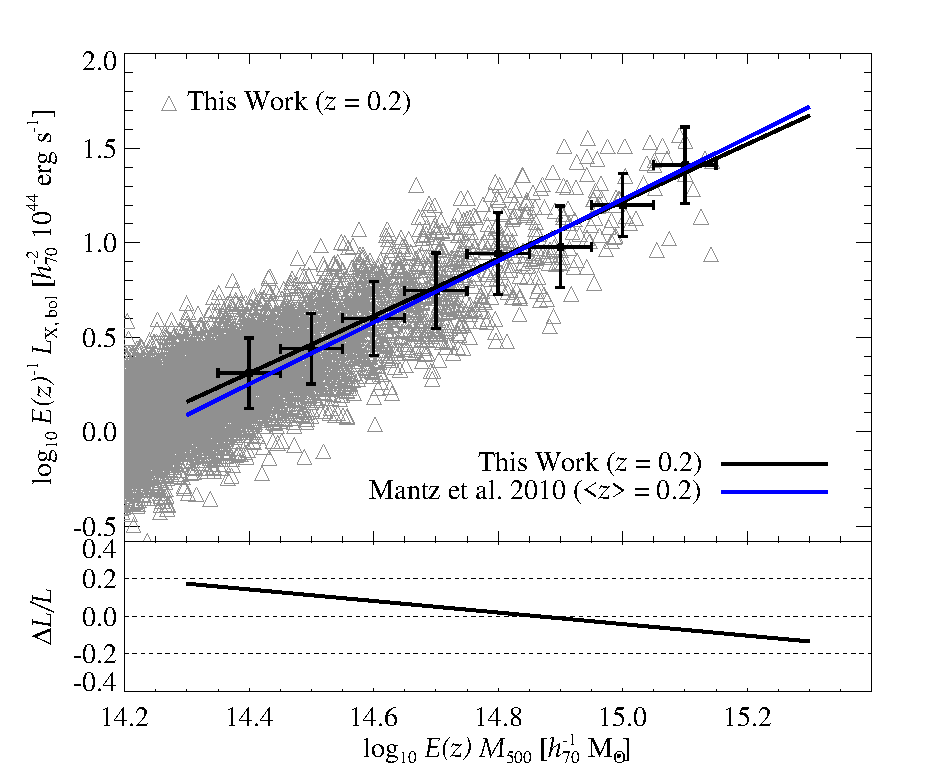
\includegraphics[width=0.48\textwidth]{figures/lx_m.eps}
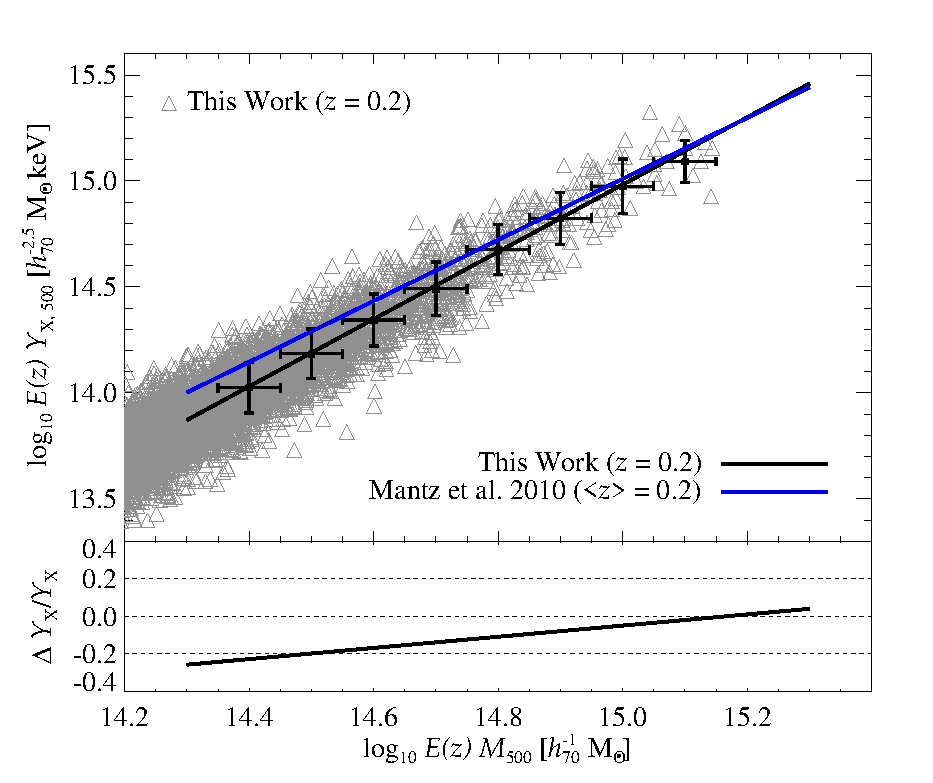
\includegraphics[width=0.48\textwidth]{figures/yx_m.eps}
%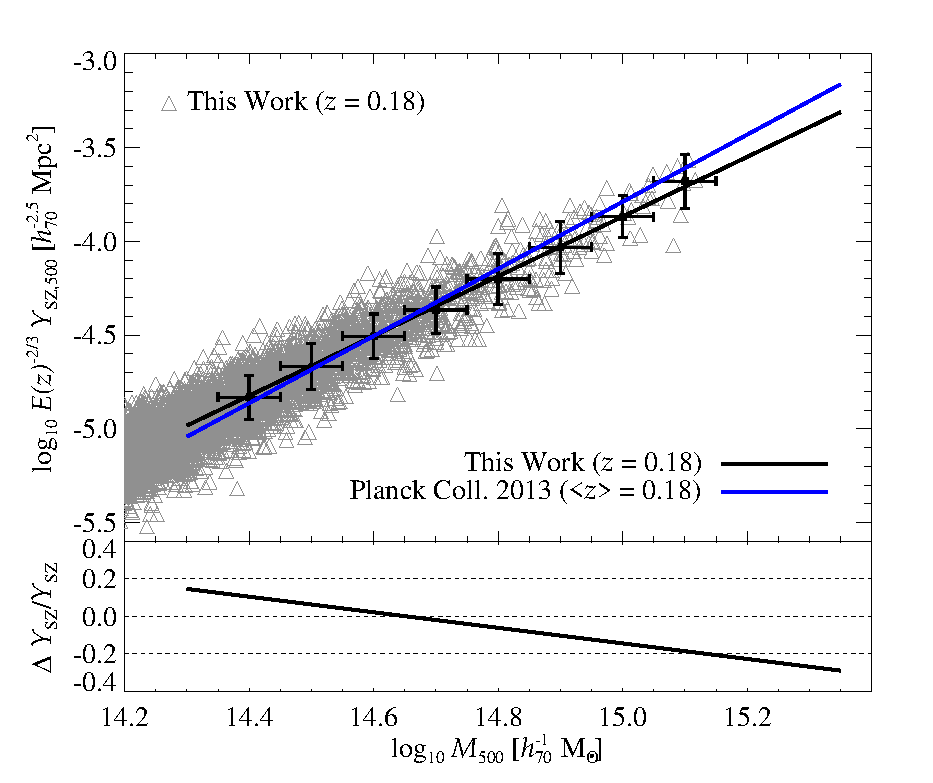
\includegraphics[width=0.33\textwidth]{figures/sz_m.eps}
\caption{X-ray scaling relations. Grey triangles show the MultiDark
  sample (limited to the mass range covered by observations), the black line is
  the corresponding scaling relation, and the blue line is the
  observational result. The black crosses represent the median values of the
  quantity in question for a given mass bin (indicated by horizontal error
  bars), and the vertical error bars represent the standard deviation within a
  bin.  \emph{Left.} We compare the bolometric X-ray luminosity-to-mass
  relation, $L_{\rmn{bol}}-M_{500}$, at $z=0.2$ to the observational sample by
  \protect\cite{2010MNRAS.406.1773M} with a median of $z \approx 0.2$. 
  \emph{Right.} $Y_{\rmn{X}}-M_{500}$ scaling relation of our model in comparison to the
  observational sample by \protect\cite{2010MNRAS.406.1773M}.} 
  %\emph{Right.} $Y_{\rmn{SZ}}-M_{500}$ scaling relation at $z=0.2$ in comparison
  %to the observational sample by the \protect\cite{2013arXiv1303.5080P} with a 
  %median redshift of about $0.18$. The bottom panels show the relative difference to
  %the observational scaling relations.}
\label{fig:X_LM}
\end{figure*}

We also account for redshift evolution of the gas profiles. While our NCCC and
CCC gas profiles as derived from the REXCESS cluster sample are merely used to
define a profile shape, the normalization of the gas profiles is set by the
observational $f_{\rmn{gas},500}-M_{500}$ relation \citep{2009ApJ...693.1142S}.
The 43 clusters used in \cite{2009ApJ...693.1142S} have redshifts $0.012 < z <
0.12$ with a \emph{median} of $z \approx 0.04$. Thus, our phenomenological gas
profile is representative of the cluster population at $z\approx0$. To extend this
profile to high-$z$, we include a \emph{self-similar} scaling of the gas density
as $\rho_{\rmn{gas}}(z) = E(z)^{2} \rho_{\rmn{gas}}(z=0)$, where $E(z)^{2} =
\Omega_{\rmn{m}} (1+z)^{3} + \Omega_{{\Lambda}}$.


%%%%%%%%%%%%%%%%%%%%%%%%%%%%%%%%%%%%%%%%%%%%%%%%%%%%%%%%%%%%%%%%%%%
%%%%%%%%%%%%%%%%%%%%%%%%%%%%%%%%%%%%%%%%%%%%%%%%%%%%%%%%%%%%%%%%%%%
\section{X-ray scaling relations and luminosity function}
\label{sec:4}

In order to check whether our phenomenologically derived gas profiles reproduce
the observations, we calculate the bolometric thermal bremsstrahlung
luminosity $L_{\rmn{bol}}$ as in \cite{1988xrec.book.....S}\footnote{We check
  our procedure by fitting each of the 31 REXCESS clusters with
  equation~(\ref{eq:gnfw}) and calculating $L_{\rmn{bol}}$ with the measured gas
  temperature of each cluster. As a result, we fall short of the observed
  luminosity by a mean (median) of about $21\%$ ($20\%$). This is reasonable
  considering that we do not permit the parameters $R_{\rmn{c}}$, $\alpha$ and
  $\delta$ to vary between different objects. Additionally, we neglect atomic
  line emission which may give a noticeable contribution, in particularly for
  low-mass clusters and in the cluster outskirts of larger systems.}  and
compare our sample result with the observed $L_{\rmn{bol}} - M_{500}$ relation
and XLF.\footnote{The mean (median) difference at $z=0$ between
  $L_{\rmn{bol}}$ within $R_{200}$ or within $R_{500}$ is $\approx 5\%$ ($\approx
  7\%$). While $L_{\rmn{bol}}$ refers to the quantity calculated within
  $R_{500}$, we note that the XLF for luminosities calculated within $R_{200}$
  will be barely changed.}

To assign a temperature to our model clusters (that is needed for calculating
$L_{\rmn{bol}}$ and $Y_{\rmn{X}}$), we adopt the $T-M_{500}$ relation by
\cite{2010MNRAS.406.1773M},
\begin{equation}
\log_{10} \left( \frac{k_{\rmn{B}}T_{\rmn{ci}}}{\rmn{keV}} \right) = 
A + B~\log_{10} \left( \frac{E(z) M_{500}}{10^{15} h_{70}^{-1} \rmn{M_{\odot}}} \right)
\label{eq:temp}
\end{equation}
where $A=0.91$, $B=0.46$, and $T_{\rmn{ci}}$ is the cluster temperature
\emph{not} centrally excised
(\citealp{2010MNRAS.406.1773M}). \cite{2010MNRAS.406.1773M} report a scatter of
$\sigma_{\rmn{yx}} = 0.06,$\footnote{Scatter is calculated as $\sigma_{\rmn{yx}}
  = \sqrt{ \left\{ \Sigma_{i=1}^{N} [Y_{i}-(A+B~X_{i})]^{2}\right\} / N-1}$
  where the sum extends over the data points $X_{i}, Y_{i}$, and $A$ and $B$ are
  the fit parameters.} which we apply to our sample using Gaussian deviates.

In the left panel of Fig.~\ref{fig:X_LM}, we show how our model
$L_{\rmn{bol}}-M_{500}$ relation compares with observations by
\cite{2010MNRAS.406.1773M} (\emph{all} data, see their Table~7). Their sample is
composed of 238 clusters at $0.02<z<0.46$ with a median of $z \approx 0.2$ and
self-consistently takes into account all selection effects, covariances,
systematic uncertainties and the cluster mass function
\citep{2010MNRAS.406.1759M}.  For this reason, we compare the
\cite{2010MNRAS.406.1773M} data to our model at $z=0.2$, and limit the
comparison to the mass range covered by the observations. Overall, there is
reassuring agreement between our phenomenological model and the data, which
probe our model most closely on scales around the cluster core radii (which is
where the contribution to $L_{\rmn{X}}$ per logarithmic interval in radius, $\dd
L_{\rmn{X}}/\dd\log r \propto r^3 n_{\rm{gas}}^2(r) \sqrt{k_{\rmn{B}}T}$,
approximately attains its maximum).  In Table~\ref{tab:LMfits}, we show our
model $L_{\rmn{bol}}-M_{500}$ scaling relation and its scatter for different
redshifts. We find that the scatter of our samples at all redshifts are Gaussian
distributed with a standard deviation of $\sigma_{yx} \approx 0.18$ that matches
the observational results of \cite{2010MNRAS.406.1773M}, which report a scatter
of $\sigma_{yx} = 0.185$.

In the right panel of Fig.~\ref{fig:X_LM}, we compare the
$Y_{\rmn{X}}-M_{500}$ relation of our sample to observational data
\citep{2010MNRAS.406.1773M}. The model agrees nicely at the high-mass end, but
underpredicts the observed scaling at low masses by about $20\%$ (at the
1-$\sigma$ level). This is the same level of deviation from the data as in the
case of $L_{\rmn{X}}$, which is more significant due to the smaller scatter in
the $Y_{\rmn{X}}$ relation. The differential contribution to the thermal energy
per logarithmic interval in radius (and hence to the integrated Compton-$y$
parameter) is given by $\dd Y /\dd\log r \propto r^3 P_{\rmn{th}}(r)$, with the
thermal gas pressure $P_{\rmn{th}}=n_{\rmn{gas}}k_{\rmn{B}}T$. It peaks at
scales slightly smaller than $R_{500}$ with 1-$\sigma$ contributions extending
out to $3\,R_{500}$ \citep{2010ApJ...725...91B}. Hence, the observational
scaling constrains our model on those large scales, quite complementary to the
X-ray luminosity. The deviations at small masses either indicates different
assumptions about $f_{\rmn{gas}}$, the gas temperature, or different selection
effects of either observational sample that we use for model calibration and
comparison.  \cite{2010MNRAS.406.1773M} determine their masses by adopting a
constant value for $f_{\rmn{gas}}$, in contrast to our approach which adopts the
observed $f_{\rmn{gas},500}-M_{500}$ relation given by
\cite{2009ApJ...693.1142S}. Additionally, we adopt the
\cite{2010MNRAS.406.1773M} \emph{centrally included} temperature throughout all
our work, while \cite{2010MNRAS.406.1773M} use the \emph{centrally excised}
temperature to calculate $Y_{\rmn{X}}$. This assumption also impacts the scatter
of the $Y_{\rmn{X}}-M$ relation. In fact, using the \emph{centrally included}
temperature, we found a scatter of $\sigma_{yx} \approx 0.11$ (see
Table~\ref{tab:YXfits} where our $Y_{\rmn{X}}$ scaling relations are reported),
significantly higher than the value of $\sigma_{yx} = 0.052$ found by
\cite{2010MNRAS.406.1773M}.

\begin{table} 
\begin{center}
\caption{$L_{\rmn{bol}}-M_{500}$ scaling relations.}
\medskip
\begin{tabular}{cccc}
\hline
\phantom{\Big|}
redshift $z$ & $A$ & $B$ & $\sigma_{yx}$ \\
\hline \\[-0.5em]
 0      & $-21.41\pm0.11$ & $1.50\pm0.01$ & 0.179\\
 0.1   & $-21.30\pm0.12$ & $1.50\pm0.01$ & 0.179\\
 0.2   & $-21.50\pm0.13$ & $1.51\pm0.01$ & 0.178\\ 
 0.4   & $-21.13\pm0.17$ & $1.49\pm0.01$ & 0.178\\ 
 0.61 & $-21.59\pm0.22$ & $1.53\pm0.01$ & 0.177\\ 
 0.78 & $-20.73\pm0.29$ & $1.48\pm0.02$ & 0.177\\ 
 1      & $-20.45\pm0.42$ & $1.46\pm0.03$ & 0.177\\[0.5em]
\hline
\end{tabular}
\label{tab:LMfits}
\end{center}
\footnotesize{Note. Scaling relations are reported in the form of $\log_{10}~(L_{\rmn{bol}}~/~E(z)~h_{70}^{-2}~10^{44}~\rmn{erg~s}^{-1})=A+B~\log_{10}~(E(z)~M_{500}~/~h_{70}^{-1}~\rmn{M_{\odot}})$. The relation scatter $\sigma_{yx}$ is also shown.}
\end{table}
 
\begin{table} 
\begin{center}
\caption{$Y_{\rmn{X}, 500}-M_{500}$ scaling relations.}
\medskip
\begin{tabular}{cccc}
\hline
\phantom{\Big|}
redshift $z$ & $A$ & $B$ & $\sigma_{yx}$ \\
\hline\\[-0.5em]
 0      & $-9.18\pm0.07$ & $1.61\pm0.01$ & 0.109\\
 0.1   & $-8.85\pm0.07$ & $1.59\pm0.01$ & 0.109\\
 0.2   & $-8.82\pm0.08$ & $1.59\pm0.01$ & 0.109\\ 
 0.4   & $-8.79\pm0.10$ & $1.59\pm0.01$ & 0.108\\ 
 0.61 & $-8.65\pm0.14$ & $1.59\pm0.01$ & 0.109\\ 
 0.78 & $-8.36\pm0.18$ & $1.57\pm0.01$ & 0.109\\ 
 1      & $-8.28\pm0.26$ & $1.57\pm0.02$ & 0.109\\[0.5em]  
\hline
\end{tabular}
\label{tab:YXfits}
\end{center}
\footnotesize{Note. Scaling relations are reported in the form of $\log_{10}~(E(z)~Y_{\rmn{X},500}~/~h_{70}^{-2.5}~\rmn{M_{\odot}}~\rmn{keV})=A+B~\log_{10}~(E(z)~M_{500}~/~h_{70}^{-1}~\rmn{M_{\odot}})$. The relation scatter $\sigma_{yx}$ is also shown.}
\end{table}


\subsection{X-ray Luminosity Function}
Studies of the XLF got out of fashion during the last years due to the
difficulties of using the X-ray luminosity for cosmological purposes. The X-ray
emissivity scales with the square of the gas density, which makes it subject to
density variations and clumping. This implies large scatter that causes a large
Malmquist bias and underlines the necessity of careful mock surveys that need to
address all systematics.

\begin{figure} 
\centering
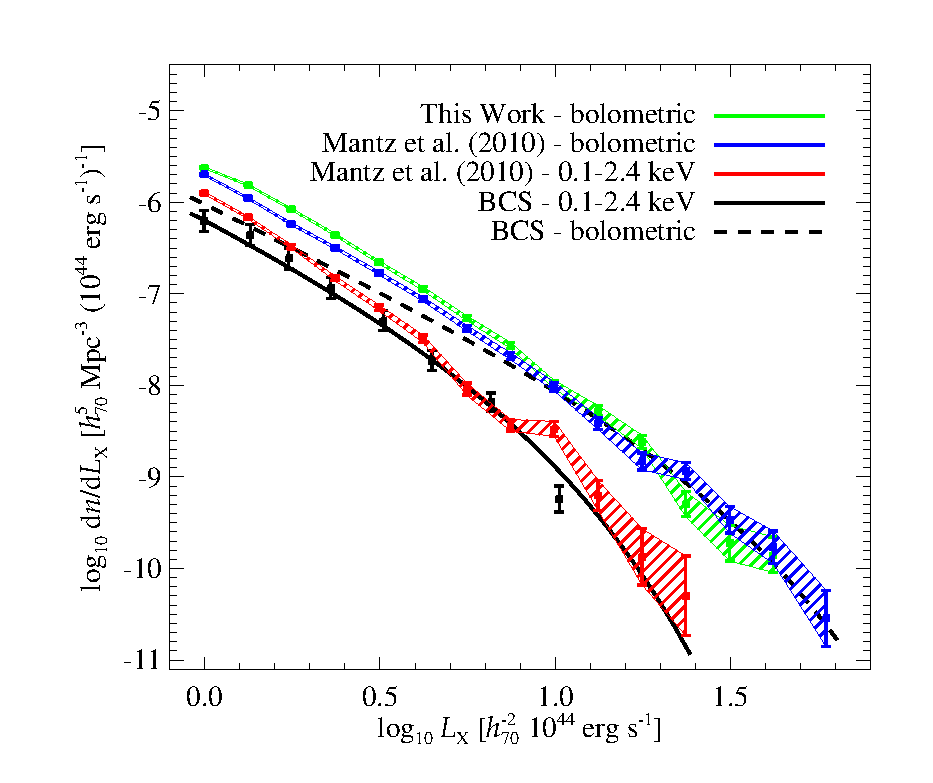
\includegraphics[width=0.48\textwidth]{figures/xlf.eps}
\caption{Bolometric and soft-band ($0.1-2.4$~keV) XLFs. Shown are the soft-band
  data points, the soft-band and bolometric Schechter fits of the BCS sample of
  \protect\cite{1997ApJ...479L.101E}, which has a median of $z \approx 0.08$.  While the
  soft-band XLF, which was obtained applying the \protect\cite{2010MNRAS.406.1773M}
  $L_{\rmn{X}}-M_{500}$ relation to the MultiDark $z = 0.1$ snapshot, compares
  well with the BCS data points, it deviates from the corresponding Schechter
  fit. We also show the bolometric XLF of \protect\cite{2010MNRAS.406.1773M} and
  bolometric XLF of our model at $z=0.1$. The XLFs are calculated in equally
  log-spaced mass bins; the error bars represent the Poissonian errors. Note
  that we limit the comparison to the luminosity range covered by our sample,
  where we cut the lowest part because in that range the XLF rapidly drops due
  to the imposed mass cut.}
\label{fig:XLF}
\end{figure}

Nevertheless, it provides a complementary check for our model. To this end, we
use the \emph{ROSAT} brightest cluster sample (BCS) XLF
\citep{1997ApJ...479L.101E}, which is in good agreement with results from the
\emph{ROSAT} ESO Flux-Limited X-ray (REFLEX; \citealp{2002ApJ...566...93B}) and
HIFLUGCS \citep{2002ApJ...567..716R}.  Note that the XLF is fully determined by
the mass function and the $L_{\rmn{X}}-M_{500}$ relation after taking into
account the observational biases. This means that applying the Malmquist and
Eddington-bias-corrected $L_{\rmn{X}}-M_{500}$ relation by
\cite{2010MNRAS.406.1773M} directly to the MultiDark mass function and
accounting for the observational scatter in $L_{\rmn{X}}-M_{500}$ should yield
an unbiased XLF. We show the resulting bolometric and soft-band ($0.1-2.4$~keV)
XLF in Fig.~\ref{fig:XLF} and compare those to the corresponding BCS XLFs and
to our model predictions. Note that there is only the Schechter fit available
for the BCS bolometric XLF.  While the soft-band XLF by
\cite{2010MNRAS.406.1773M} agrees well with the BCS data points, it deviates
from the corresponding Schechter fit at low luminosities. This is also true in
the bolometric band, where the XLFs of \cite{2010MNRAS.406.1773M} and our model
agree well, but deviate from the BCS Schechter fit at low luminosities. This may
be an artifact due to the use of Schechter fit instead of the data points or may
point to incompleteness of the BCS sample. Note that the Poissonian errors of
the XLF obtained from the MultiDark simulation are a lower limit as we are
neglecting the uncertainty due to cosmic variance.  Studies of the XLF will
become again an important topic with the upcoming launch of the \emph{e}ROSITA
satellite (e.g., \citealp{2011MSAIS..17..159C}) and further studies in this
direction are desirable. For these reasons, we do not show XLF predictions at
other redshifts, leaving this for a future study.


%%%%%%%%%%%%%%%%%%%%%%%%%%%%%%%%%%%%%%%%%%%%%%%%%%%%%%%%%%%%%%%%%%%
%%%%%%%%%%%%%%%%%%%%%%%%%%%%%%%%%%%%%%%%%%%%%%%%%%%%%%%%%%%%%%%%%%%
\section{SZ scaling relations}
\label{sec:5}
In the right panel of Fig.~\ref{fig:X_LM}, we compare the
$Y_{\rmn{SZ}}-M_{500}$ relation in our model (calculated as in equation~(3) of
\citealp{2011arXiv1109.3709B}) with the observed scaling relation by the
\cite{2013arXiv1303.5080P}. {\bf We compare with the result obtained from the 
\emph{Planck} COSMO sample with Malmquist bias correction (see their Table~A.1),
which has a median redshift of $0.18$. Hence, we compare the data to our relation 
at the MultiDark snapshot $z=0.2$}. Our model reproduces the data remarkably well, except 
for the high-mass end where our simulations have a weaker constraining power due to the 
smaller box size in comparison to the survey volume of {\em Planck}. We find a scatter of
$\sigma_{yx} \approx 0.11$ which compares well with the \emph{Planck} result of
$\sigma_{yx} \approx 0.08$. In Table~\ref{tab:YSZfits}, we report our SZ scaling
relations for different redshifts.

\begin{figure} 
\centering
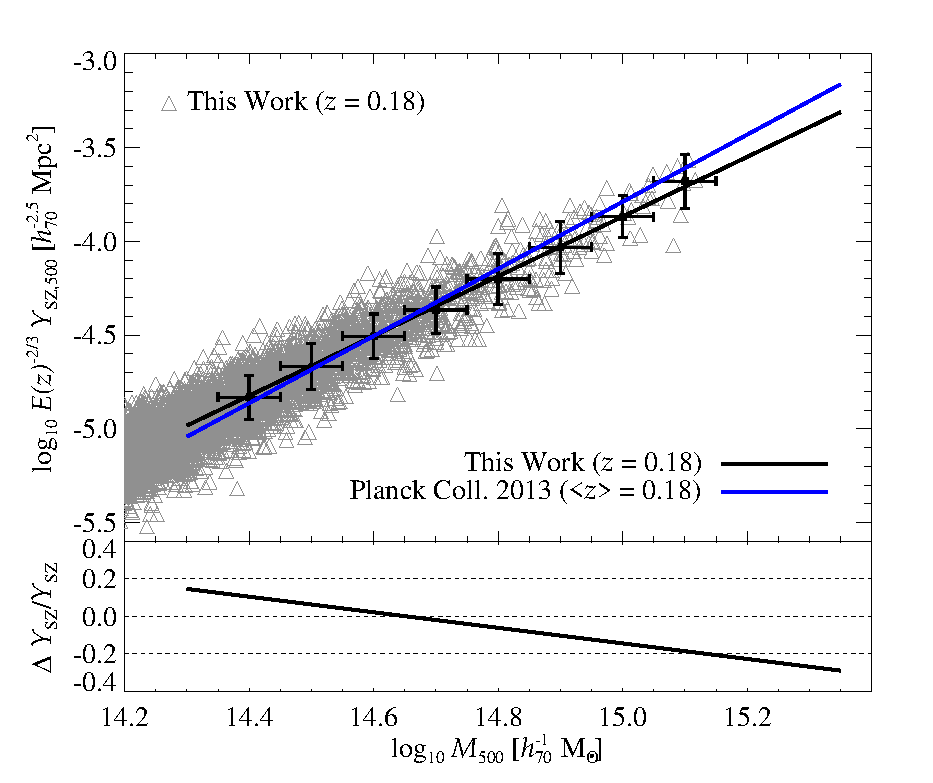
\includegraphics[width=0.48\textwidth]{figures/sz_m.eps}
\caption{SZ scaling relations. Grey triangles show the MultiDark
  sample (limited to the mass range covered by observations), the black line is
  the corresponding scaling relation, and the blue line is the
  observational result. The black crosses represent the median values of the
  quantity in question for a given mass bin (indicated by horizontal error
  bars), and the vertical error bars represent the standard deviation within a
  bin.  \emph{Left.} We compare the bolometric X-ray luminosity-to-mass
  relation, $L_{\rmn{bol}}-M_{500}$, at $z=0.2$ to the observational sample by
  \protect\cite{2010MNRAS.406.1773M} with a median of $z \approx 0.2$. 
  \emph{Right.} $Y_{\rmn{X}}-M_{500}$ scaling relation of our model in comparison to the
  observational sample by \protect\cite{2010MNRAS.406.1773M}. 
  \emph{Left.} $Y_{\rmn{SZ}}-M_{500}$ scaling relation at $z=0.2$ in comparison
  to the observational sample by the \protect\cite{2013arXiv1303.5080P} with a 
  median redshift of about $0.18$. The bottom panels show the relative difference to
  the observational scaling relations.}
\label{fig:SZ_M}
\end{figure}

\begin{figure*} 
\centering
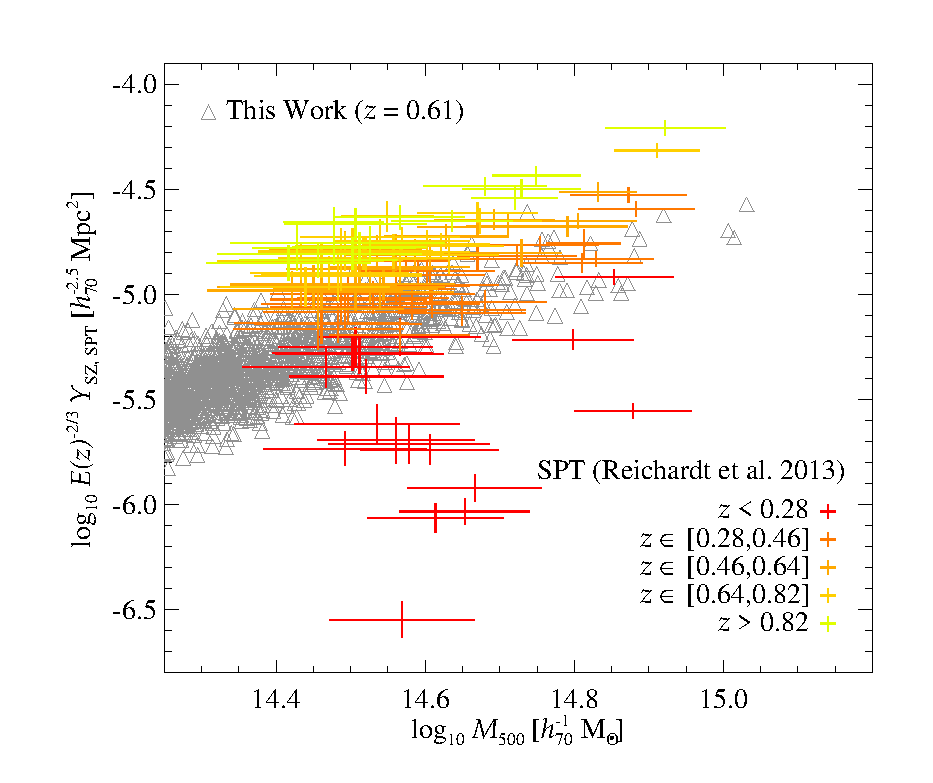
\includegraphics[width=0.48\textwidth]{figures/sz_m_SPT.eps}
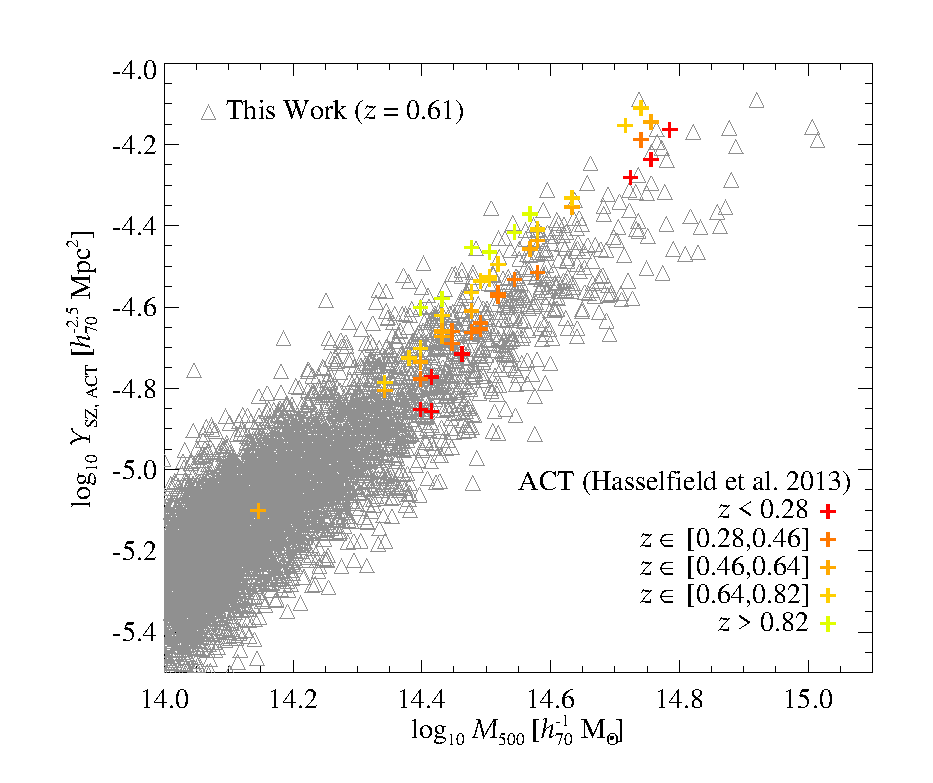
\includegraphics[width=0.48\textwidth]{figures/sz_m_ACT.eps}
\caption{SZ scaling relations. Grey triangles show the MultiDark
  sample (limited to the mass range covered by observations), the black line is
  the corresponding scaling relation, and the blue line is the
  observational result. The black crosses represent the median values of the
  quantity in question for a given mass bin (indicated by horizontal error
  bars), and the vertical error bars represent the standard deviation within a
  bin.  \emph{Left.} We compare the bolometric X-ray luminosity-to-mass
  relation, $L_{\rmn{bol}}-M_{500}$, at $z=0.2$ to the observational sample by
  \protect\cite{2010MNRAS.406.1773M} with a median of $z \approx 0.2$. 
  \emph{Right.} $Y_{\rmn{X}}-M_{500}$ scaling relation of our model in comparison to the
  observational sample by \protect\cite{2010MNRAS.406.1773M}. 
  \emph{Left.} $Y_{\rmn{SZ}}-M_{500}$ scaling relation at $z=0.2$ in comparison
  to the observational sample by the \protect\cite{2013arXiv1303.5080P} with a 
  median redshift of about $0.18$. The bottom panels show the relative difference to
  the observational scaling relations.}
\label{fig:SZ_M_1}
\end{figure*}

\begin{table} 
\begin{center}
\caption{$Y_{\rmn{SZ}, 500}-M_{500}$ scaling relations.}
\medskip
\begin{tabular}{cccc}
\hline
\phantom{\Big|}
redshift $z$ & $A$ & $B$ & $\sigma_{yx}$ \\
\hline\\[-0.5em]
 0      & $-27.93\pm0.07$ & $1.60\pm0.01$ & 0.109\\
 0.1   & $-27.74\pm0.07$ & $1.59\pm0.01$ & 0.109\\
 0.18 & $-27.73\pm0.08$ & $1.59\pm0.01$ & 0.109\\
 0.2   & $-27.65\pm0.08$ & $1.59\pm0.01$ & 0.109\\ 
 0.4   & $-27.57\pm0.10$ & $1.59\pm0.01$ & 0.108\\ 
 0.61 & $-27.50\pm0.13$ & $1.59\pm0.01$ & 0.109\\ 
 0.78 & $-27.15\pm0.18$ & $1.58\pm0.01$ & 0.109\\ 
 1      & $-27.01\pm0.26$ & $1.58\pm0.02$ & 0.109\\[0.5em] 
\hline
\end{tabular}
\label{tab:YSZfits}
\end{center}
\footnotesize{Note. Scaling relations are reported in the form of $\log_{10}~(E(z)^{-2/3}~Y_{\rmn{SZ},500}~/~h_{70}^{-2.5}~\rmn{Mpc}^{2})=A+B~\log_{10}~(M_{500}~/~h_{70}^{-1}~\rmn{M_{\odot}})$. The relation scatter $\sigma_{yx}$ is also shown.}
\end{table}

{\bf We additionally compare our $Y_{\rmn{SZ}}$ to the results from the South Pole Telescope (SPT) 
and Atacama Cosmology Telescope (ACT) surveys.
We select a subsample of SPT clusters from \cite{2013ApJ...763..127R}, formed by the
115 objects with confirmed redshift and signal-to-noise above 5, which has a median
redshift of 0.56 with rms of 0.27. \cite{2013ApJ...763..127R} provide $Y_{\rmn{SZ}}$ 
within an aperture of $1'$, corresponding to a median radius of $0.2$~h$_{70}^{-1}$~Mpc 
at $z = 0.56$, which we use as aperture to calculate $Y_{\rmn{SZ, SPT}}$ in our MultiDark sample.

In the left panel of Fig.~\ref{fig:SZ_M_1}, we compare the SPT cluster subsample to our 
scaling relation at the three different MutliDark snapshots of $z = 0.4$, $0.61$ 
and $0.78$. We color-coded the SPT clusters in order to show that the SPT 
selection function is nearly redshift-independent. The fact that the angular size of galaxy clusters 
decreases with redshift is an advantage for SPT due to its small beam, in fact, higher-redshift clusters 
are less confused by primary CMB fluctuations. This effect is inverse for \emph{Planck} due to its
larger beam. We can conclude that while our $Y_{\rmn{SZ}}-M_{500}$ scaling relation 
compare fairly well to the median SPT cluster population, the SPT sample has a too
large scatter to be well represented by single MultiDark snapshots.

In the right panel of Fig.~\ref{fig:SZ_M_1}, we compare our scaling relation to
the ACT sample overlapping with the Sloan Digital Sky Survey stripe 82 
(\citealp{2013JCAP...07..008H}; we use the quantities inferred from the
universal pressure profile scaling relation).
The sample has a median redshift of 0.58 with rms of 0.28.
\cite{2013JCAP...07..008H} provides $Y_{\rmn{SZ}}$ within $R_{500}$ which
median, $0.42$~h$_{70}^{-1}$~Mpc, is, however, almost half of ours at the
MultiDark snapshot $z=0.61$. Therefore, we use an aperture of $0.42$~h$_{70}^{-1}$~Mpc
to calculate our $Y_{\rmn{SZ, ACT}}$. Also in this case we can conclude
that our mock sample reproduce fairly well the median observational sample. 
Note, however, the very different scatter of SPT and ACT samples.} 

%%%%%%%%%%%%%%%%%%%%%%%%%%%%%%%%%%%%%%%%%%%%%%%%%%%%%%%%%%%%%%%%%%%
%%%%%%%%%%%%%%%%%%%%%%%%%%%%%%%%%%%%%%%%%%%%%%%%%%%%%%%%%%%%%%%%%%%
\section{Conclusions}
\label{sec:6}

{\bf Discussion...}

{\bf We build a complete cosmological sample of galaxy clusters from the MultiDark 
$N$-body simulation with redshifts ranging from $z = 0$ to 1. We construct a 
\emph{phenomenological} model for the cluster-gas distribution. This is characterized 
by X-ray-inferred (CCC and NCCC) gas profiles (taken from the REXCESS sample) 
and a cluster-mass-dependent gas fraction. We assign such a (cluster mass-dependent) 
gas density profile to each DM halo in our sample and sort it into the NCCC/CCC populations 
according to a dynamical disturbance parameter that is calculated from the DM distribution.
With this model, we obtain a cosmologically complete mock catalog of galaxy
clusters that matches the observed $L_{\rmn{X, bol}}$-to-$M_{500}$,
$Y_{\rmn{X}}$-to-$M_{500}$, and $Y_{\rmn{SZ}}$-to-$M_{500}$ relations, as well
as the X-ray luminosity function. We apply it in the companion Paper~2 to 
predict the radio and gamma-ray emission of our sample. 

Eventually, we provide a cosmologically complete multi-frequency mock catalog for the (non-)thermal 
cluster emission at different redshifts. We make these catalogs publicly and freely available 
on-line through the MultiDark database (www.multidark.org). Those contain the quantities
$\rho_{\rmn{gas}}$, $L_{\rmn{X, bol}}$, $Y_{\rmn{X}}$, $Y_{\rmn{SZ}}$, $L_{120~\rmn{MHz}}$, 
$L_{1.4~\rmn{GHz}}$, $L_{>100~\rmn{MeV}}$ and $L_{>100~\rmn{GeV}}$ (among many others). 
We hope that the community can make valuable use of these catalogues in synergy with the future 
radio, X-ray and gamma-ray data.}


%%%%%%%%%%%%%%%%%%%%%%%%%%%%%%%%%%%%%%%%%%%%%%%%%%%%%%%%%%%%%%%%%%%
%%%%%%%%%%%%%%%%%%%%%%%%%%%%%%%%%%%%%%%%%%%%%%%%%%%%%%%%%%%%%%%%%%%
\section*{Acknowledgments}
We thank Anders Pinzke for many useful discussions. We also thank Harald Ebeling, 
Stefan Gottl{\"o}berg, Anatoly Klypin, Andrey Kravtsov, Adam Mantz, Frazer Pearce, 
Jos\'e Alberto Rubi\~no, and Gustavo Yepes, for the useful discussions and advices. 
Finally, we thank the MultiDark database people, in particular Adrian Partl and Kristin Riebe. 
F.Z.{\ }acknowledges the CSIC financial support as a JAE-Predoc grant of the 
program ``Junta para la Ampliaci\'on de Estudios'' co-financed by the FSE. 
F.Z.{\ }acknowledges the hospitality of the Leiden Observatory during his stay.
F.Z.{\ }and F.P.{\ } thank the support of the Spanish MICINN's Consolider-Ingenio 2010 Programme under
grant MultiDark CSD2009-00064. C.P.{\ }gratefully acknowledges financial support
of the Klaus Tschira Foundation. The MultiDark Database used in this paper and
the web application providing online access to it were constructed as part of
the activities of the German Astrophysical Virtual Observatory as result of a
collaboration between the Leibniz-Institute for Astrophysics Potsdam (AIP) and
the Spanish MultiDark Consolider Project CSD2009-00064. The Bolshoi and
MultiDark simulations were run on the NASA's Pleiades supercomputer at the NASA
Ames Research Center.


%%%%%%%%%%%%%%%%%%%%%%%%%%%%%%%%%%%%%%%%%%%%%%%%%%%%%%%%%%%%%%%%%%%
%%%%%%%%%%%%%%%%%%%%%%%%%%%%%%%%%%%%%%%%%%%%%%%%%%%%%%%%%%%%%%%%%%%
\bibliographystyle{mn2e}
\bibliography{bib_file}


%%%%%%%%%%%%%%%%%%%%%%%%%%%%%%%%%%%%%%%%%%%%%%%%%%%%%%%%%%%%%%%%%%
%%%%%%%%%%%%%%%%%%%%%%%%%%%%%%%%%%%%%%%%%%%%%%%%%%%%%%%%%%%%%%%%%%
\label{lastpage}

\end{document}


